\documentclass[fleqn,a4paper,12pt]{article}

%used Packages
\usepackage{standalone}		% Zum Einlesen aus anderen .tex-Files
\usepackage{geometry}		% Zur Bearbeitung des Layouts (Ränder,...)
\usepackage[german]{babel}
\usepackage[utf8]{inputenc}
\usepackage{amsmath}		% Mathematische Symbole
\usepackage{amssymb}     	% Nochmehr mathematische Symbole
\usepackage{dsfont}      	% Schriftsatz fuer Zahlenmengensymbole
%\usepackage{verbatim}   	% erweiterte Verbatim-Umgebung
\usepackage{alltt}       	% Quasi-Verbatim-Umgebung
\usepackage{fancyhdr}    	% Eigene Kopfzeilen
\usepackage{graphicx}    	% Zum Einbinden von Grafiken
							% Einbinden einer eps-Grafik geht so: includegraphics{path}
\usepackage{wrapfig}
\usepackage{lscape}
\usepackage{rotating}
\usepackage{epstopdf}

% Skalierung der Grafiken
\setlength{\unitlength}{1cm}

\frenchspacing               % Kein Extrafreiraum nach Satzzeichen
\setlength{\parindent}{0pt}  % Neue Absaetze nicht einruecken
%\sloppy                     % Schlampige Absatzformatierung
\fussy                       % Penible Absatzformatierung
\linespread{1.5}             % Zeilenabstand


% Seitenraender
\geometry{left=30mm, right=40mm, bottom=30mm}
				% Doc-class, Packageimports, fancy stuff
%Seitenränder formatieren
\addtolength{\voffset}{-2cm}
\addtolength{\textheight}{0cm}
\addtolength{\hoffset}{0cm}
\addtolength{\textwidth}{2cm}
\addtolength{\headheight}{2cm} % fuer jeden Strichkode einen Zentimeter

% Font fuer Code 39
\font\xlix=wlc39 scaled 1200
\newcommand\barcode[1]{{\xlix@#1@}}

% Name, Matrikelnummer, Barcode
\newcommand\student[2]{
	\mbox{\scriptsize
		\begin{tabular}{@{}l@{}r@{}}
			\multicolumn{2}{@{}r@{}}{\barcode{#2}}\\
			#1&#2\\
		\end{tabular}}}

% Kopfzeile
\pagestyle{fancy}            % Eigene Kopfzeilen verwenden
\lhead{
	\small
	\textsc{Grundlagen der Signalverarbeitung \\
		WS 2017/2018 \\
		\"Ubung (\today)}
	\vfill}
\rhead{
	\begin{tabular}[b]{@{}rr@{}}
		\student{Philipp Badenhoop}{572693} &
		\student{Steven Lange}{568733} \\
		\student{Pascal Jochmann}{575056} &
		\student{Kevin Trogant}{572451}
\end{tabular}}			% Definition der Kopfzeile
%andere Definitionen
\providecommand{\R}{{\mathbb R}}
\providecommand{\N}{{\mathbb N}}
\providecommand{\Z}{{\mathbb Z}}
\providecommand{\Q}{{\mathbb Q}}
\providecommand{\C}{{\mathbb C}}
\providecommand{\F}{\mathcal{F}}
\providecommand{\less}{\setminus}
\providecommand{\inv}{{}^{-1}}
\providecommand{\Land}{\bigwedge}
\providecommand{\Lor}{\bigvee}			% Liste der zusätzlichen Commands und redefines

\begin{document}
	\section*{Übungsaufgabe 18:}
	
	\begin{tabular}{c c | c c c c | c }
			& n				& 0					& 1			& 2					& \multicolumn{2}{l}{3}\\
		\cline{2-6}
			& $t_n$			& -1				& 0			& 1					& \multicolumn{2}{l}{2}\\
			& $f_n$			& 1					& 0			& 1					& \multicolumn{2}{l}{2}\\
		m	&$\varphi_m$	&					&			&					&							&$\sum_{n=0}^{N-1}$\\
		\cline{1-7}	
		0	& $e^0$			& 1 				& 1			& 1					& 1							& 4\\
		1	& $e^{t_n}$		& $\frac{1}{e}$		& 1			& $e$				& $e^2$						& 11,47\\
		2	& $e^{-t_n}$		& $e$				& 1			& $\frac{1}{e}$		& $\frac{1}{e^2}$			& 4,22\\
		\cdashline{1-7}
			& $e^{2t_n}$	& $\frac{1}{e^2}$	& 1			& $e^2$				& $e^4$						& 63,12\\
			& $e^{-2t_n}$	& $e^2$				& 1			& $\frac{1}{e^2}$	& $\frac{1}{e^4}$			& 8,54
	\end{tabular}\\
	Mit der folgenden Gleichung
	\begin{align*}
		\left(\begin{matrix}
			a_{00}	&	\dots	& a_{0,m-1}\\
			\vdots	&			& \vdots\\
			a_{m-1,0}	&	\dots	& a_{m-1,m-1}
		\end{matrix}\right)\cdot \left(\begin{matrix}c_0\\\vdots\\c_{m-1}\end{matrix}\right) = 
		\left(\begin{matrix}
			\sum_{n=0}^{N-1} \varphi_0(t_n)\cdot f(t_n)\\
			\vdots\\
			\sum_{n=0}^{N-1} \varphi_{m-1}(t_n)\cdot f(t_n)\\
		\end{matrix}\right)
	\end{align*}
	mit $a_{i,j}:= \sum_{n=0}^{N-1}\varphi_i(t_n)\cdot \varphi_j(t_n)$ ergibt sich daraus:
	\begin{align*}
		\left(\begin{matrix}c_0\\c_1\\c_2\end{matrix}\right) = 
		\left(\begin{matrix}
			4		&	11,47	& 4,22\\
			11,47	&	63,12	& 4\\
			4,22	&	4		& 8,54
		\end{matrix}\right)^{-1} \cdot
		\left(\begin{matrix}
			2\\
			17,13\\
			-2,08\\
		\end{matrix}\right) \approx 
		\left(\begin{matrix}
			0,5\\
			0,22\\
			-0,59
		\end{matrix}\right)
	\end{align*}
	Damit ergibt sich für $f_{app}(t) = -0,59 e^{-t}+0,22 e^{t}+0,5$ folgendes Fehlermaß
	\begin{align*}
		E^2(c) = \sum_{i=0}^3 \left[ f(t_n) - f_{app}(t_n)\right]^2 = 4,092 + 0,017 + 0,014 + 0,002 = 4,125
	\end{align*}
	
	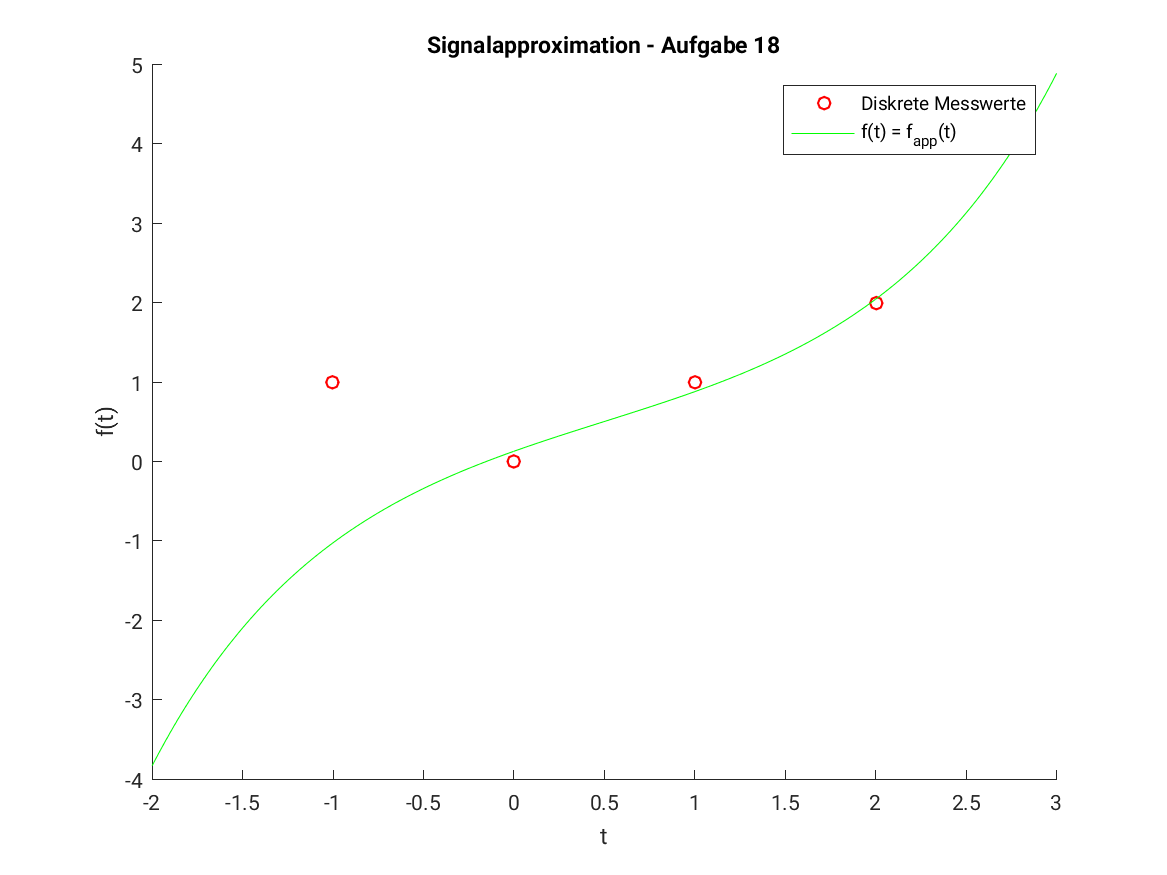
\includegraphics[scale = 0.8]{A18_functionPlot.png}
\newpage
	\section*{Übungsaufgabe 19:}
	a) \newline
	\begin{align*}
	\left(\begin{matrix}c_0\\c_1\\c_2\end{matrix}\right) =
	\left(\begin{matrix}
			6.00 & -1.27 & 1.20 & \\
			-1.27 & 3.60 & -0.58 & \\
			1.20 & -0.58 & 3.87 & \\
	\end{matrix}\right)^{-1} \cdot
	\left(\begin{matrix}
			27.00\\
			-20.61\\
			11.64\\
	\end{matrix}\right) \approx
	\left(\begin{matrix}
			3.31\\
			-4.34\\
			1.33\\
	\end{matrix}\right)
	\end{align*}
	$f_{app}(t) = 3.31 \cdot cos(0) + -4.34 \cdot cos(t) + 1.33 \cdot cos(2t) $
	\begin{align*}
			E^2(c) = \sum_{i=0}^5 \left[ f(t_n) - f_{app}(t_n)\right]^2 = 0.58
	\end{align*}

	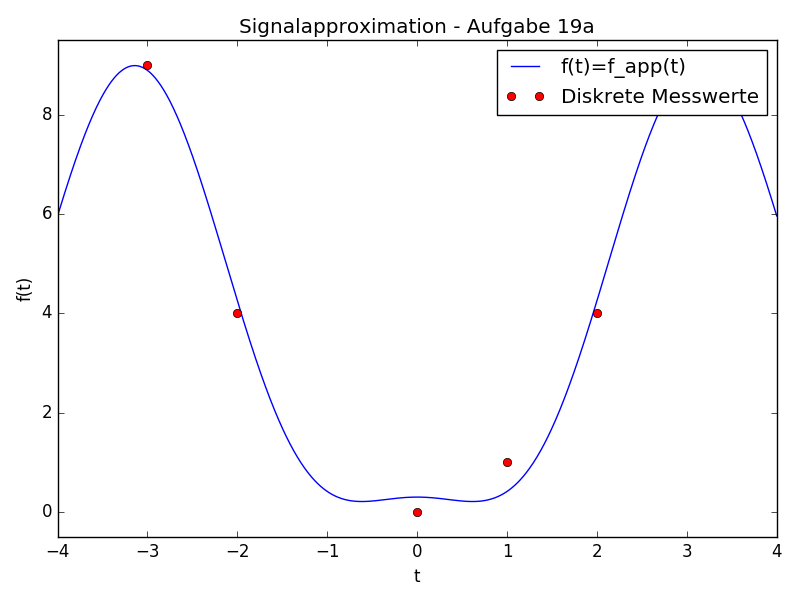
\includegraphics[scale=0.8]{A19a.png}

	b) \newline
	\begin{align*}
	\left(\begin{matrix}c_0\\c_1\\c_2\end{matrix}\right) =
	\left(\begin{matrix}
			6.00 & 0.84 & 0.91 & \\
			0.84 & 2.40 & -0.69 & \\
			0.91 & -0.69 & 2.13 & \\
	\end{matrix}\right)^{-1} \cdot
	\left(\begin{matrix}
			27.00\\
			0.84\\
			0.91\\
	\end{matrix}\right) \approx
	\left(\begin{matrix}
			5.18\\
			-2.18\\
			-2.50\\
	\end{matrix}\right)
	\end{align*}
	$f_{app}(t) = 5.18 \cdot sin(\frac{\pi}{2}) + -2.18 \cdot sin(t) + -2.50 \cdot sin(2t) $
	\begin{align*}
			E^2(c) = \sum_{i=0}^5 \left[ f(t_n) - f_{app}(t_n)\right]^2 = 59.13
	\end{align*}

	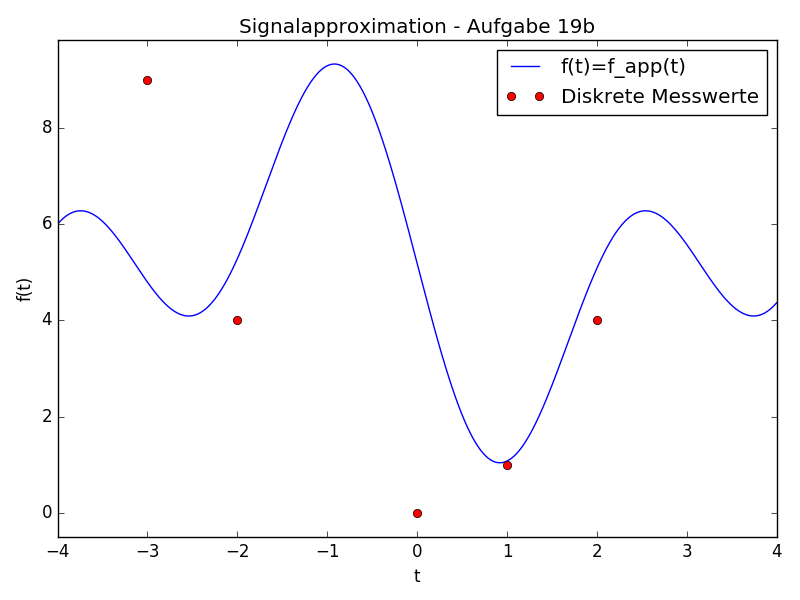
\includegraphics[scale=0.8]{A19b.png}

	c) \newline
	zu a) Punkt (-1,1) hinzugefügt: \newline
	\begin{align*}
	\left(\begin{matrix}c_0\\c_1\\c_2\end{matrix}\right) =
	\left(\begin{matrix}
			7.00 & -0.73 & 0.78 & \\
			-0.73 & 3.89 & -0.81 & \\
			0.78 & -0.81 & 4.04 & \\
	\end{matrix}\right)^{-1} \cdot
	\left(\begin{matrix}
			28.00\\
			-20.07\\
			11.22\\
	\end{matrix}\right) \approx
	\left(\begin{matrix}
			3.41\\
			-4.25\\
			1.27\\
	\end{matrix}\right)
	\end{align*}
	$f_{app}(t) = 3.41 \cdot cos(0) + -4.25 \cdot cos(t) + 1.27 \cdot cos(2t) $\begin{align*}
			E^2(c) = \sum_{i=0}^5 \left[ f(t_n) - f_{app}(t_n)\right]^2 = 0.82
	\end{align*}

	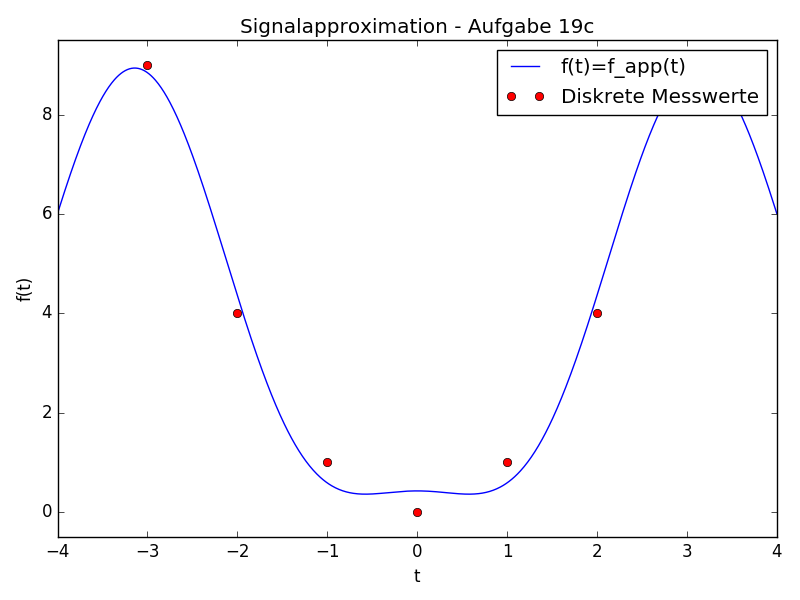
\includegraphics[scale=0.8]{A19c1.png}

	zu b) Punkt (-1,1) hinzugefügt: \newline
	\begin{align*}
	\left(\begin{matrix}c_0\\c_1\\c_2\end{matrix}\right) =
	\left(\begin{matrix}
			7.00 & 0.00 & 0.00 & \\
			0.00 & 3.11 & 0.08 & \\
			0.00 & 0.08 & 2.96 & \\
	\end{matrix}\right)^{-1} \cdot
	\left(\begin{matrix}
			28.00\\
			0.00\\
			0.00\\
	\end{matrix}\right) \approx
	\left(\begin{matrix}
			4.00\\
			0.00\\
			-0.00\\
	\end{matrix}\right)
	\end{align*}
	$f_{app}(t) = 4.00 \cdot sin(\frac{\pi}{2} + 0.00 \cdot sin(t) + -0.00 \cdot sin(2t) $\begin{align*}
			E^2(c) = \sum_{i=0}^5 \left[ f(t_n) - f_{app}(t_n)\right]^2 = 84.00
	\end{align*}

	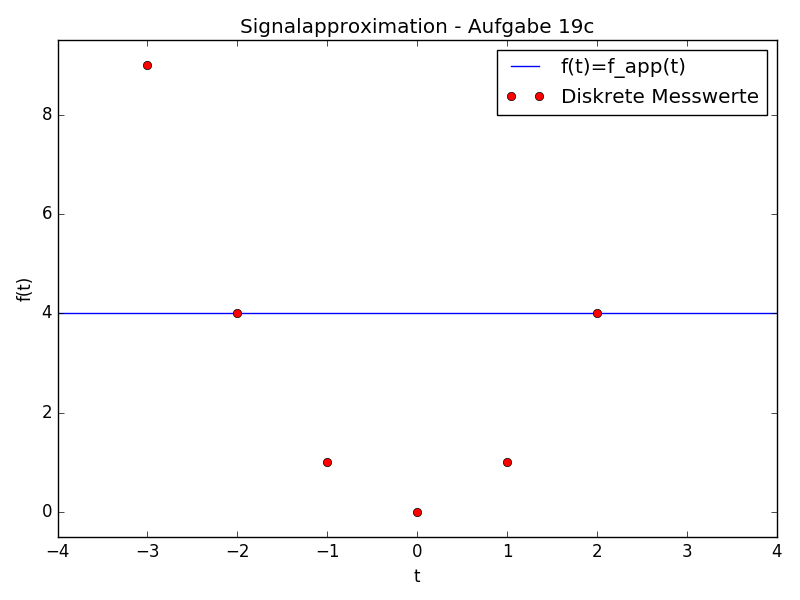
\includegraphics[scale=0.8]{A19c2.png}

	Zusammenfassung: \newline
	Während in a) sich kaum etwas am quadratischen Fehler sowie der Approximationsfunktion ändert, verändert sich die Approximationsfunktion in c) zu einer konstanten Funktion.

\newpage
    \section*{Übungsaufgabe 20}
    Messerte: \\
    \begin{tabular}{|c|c|c|c|c|c|c|}
        \hline
        $\mathbf{n}$   & 0 & 1 & 2 & 3   & 4 & 5 \\
        \hline
        $\mathbf{t_n}$ & 0 & 1 & 2 & 3   & 4 & 5 \\
        \hline
        $\mathbf{f_n}$ & 2 & 4 & 3 & 3.5 & 5 & 4 \\
        \hline
    \end{tabular} \\
    Wir wollen die Funktion $f_{ap}(t) = c_2 t^2 + c_1 t + c_0$ aufstellen.
    \begin{align*}
        \begin{bmatrix}
            \sum_{n=0}^{5} t_n^{0} t_n^{0} &
            \sum_{n=0}^{5} t_n^{0} t_n^{1} &
            \sum_{n=0}^{5} t_n^{0} t_n^{2} \\
            \sum_{n=0}^{5} t_n^{1} t_n^{0} &
            \sum_{n=0}^{5} t_n^{1} t_n^{1} &
            \sum_{n=0}^{5} t_n^{1} t_n^{2} \\
            \sum_{n=0}^{5} t_n^{2} t_n^{0} &
            \sum_{n=0}^{5} t_n^{2} t_n^{1} &
            \sum_{n=0}^{5} t_n^{2} t_n^{2} \\
        \end{bmatrix}
        \begin{bmatrix}
            c_{0} \\
            c_{1} \\
            c_{2} \\
        \end{bmatrix}
        &=
        \begin{bmatrix}
            \sum_{n=0}^{5} f_n t_n^{0}\\
            \sum_{n=0}^{5} f_n t_n^{1}\\
            \sum_{n=0}^{5} f_n t_n^{2}\\
        \end{bmatrix}
        \\
        6 c_{0} +
        15 c_{1} +
        55 c_{2} &=
        9\\
        15 c_{0} +
        55 c_{1} +
        225 c_{2} &=
        10\\
        55 c_{0} +
        225 c_{1} +
        979 c_{2} &=
        16\\
    \end{align*}
    Lösen (zB. mittels Gauß-Algorithmus) ergibt: $c_0 = \frac{41}{14} c_1 = -\frac{5}{28} c_2 = -\frac{3}{28}$ \\
    Als quadratischer Fehler ergibt sich dann:
    \begin{align*}
        E^2(c) &= \sum_{n=0}^{5} \left[ f_n - c_0 t_n^0 - c_1 t_n^1 - c_2 t_n^2 \right]^2 \\
               &= \sum_{n=0}^{5} \left[ f_n - \frac{41}{14} + \frac{5}{28} t_n + \frac{3}{28} t_n^2 \right]^2 \\
        \textit{Einsetzen: } \; &\approx 60.65 
    \end{align*}
\newpage
    \section*{Übungsaufgabe 21}
    \begin{align*}
        \int_{-1}^{1} t_n t_n^2 \, dt = \left[ \frac{t^4}{4} \right]_{-1}^{1} = 0
    \end{align*}
    $t_n \cdot t_n^2$ ist ungerade. Für symmetrische Grenzen verschwindet die Fläche unterm untegeraden Integral.
    \begin{align*}
        \sum_{n=0}^{N-1} t_n \cdot t_n^2 &= -1 \cdot (-1)^2 + -0.5 \cdot (-0.5)^2 + 0 \cdot 0^2 + 0.5 \cdot 0.5^2 + 1 \cdot 1^2
            & = 0
    \end{align*}
    Die Basisfunktionen sind orthogonal.
\newpage\end{document}